%%% Décommenter pour une présentation
\documentclass{beamer}
%%%

%%% Décommenter pour avoir un article
%\documentclass[handout]{beamer}
%\usepackage{pgfpages}
%\pgfpagesuselayout{2 on 1}[a4paper,border shrink=5mm]
%\setbeameroption{show notes on second screen=bottom} % Beamer manual, section 19.3
%%%

%%%%%%%%%%%%%%%%%%%%%%%%%%%%%%%%%%%%%%%%%%%%%%%%%%%%%%%%%%%%%%%%%%%%%%
% NE PAS MODIFIER CETTE PARTIE

\usetheme{Warsaw}
\usepackage[utf8]{inputenc}
\usepackage[T1]{fontenc}
\usepackage{amsmath}
\usepackage{amsfonts}
\usepackage{amssymb}
\usepackage{graphicx}
\usepackage{listings}
\usepackage{hyperref}
\usepackage{tikz}
\usepackage{verbatim}
\usetikzlibrary{arrows,shapes}

\graphicspath{{graphics/}}

\hypersetup{pdfstartview={Fit}}



\AtBeginSection[]{
  \begin{frame}
  \vfill
  \centering
  \begin{beamercolorbox}[sep=8pt,center,shadow=true,rounded=true]{title}
    \usebeamerfont{title}\insertsectionhead\par%
  \end{beamercolorbox}
  \vfill
  \end{frame}
}

\setbeamertemplate{note page}[plain] % Beamer manual, section 19.1
\newlength{\parskipbackup}
\setlength{\parskipbackup}{\parskip}
\newlength{\parindentbackup}
\setlength{\parindentbackup}{\parindent}
\newcommand{\baselinestretchbackup}{\baselinestretch}
\usetemplatenote{\rmfamily \scriptsize%
  \setlength{\parindent}{1em} \setlength{\parskip}{1ex}%
  \renewcommand{\baselinestretch}{1}%
  \noindent \insertnote%

  \setlength{\parskip}{\parskipbackup}%
  \setlength{\parindent}{\parindentbackup}%
  \renewcommand{\baselinestretch}{\baselinestretchbackup}%
}

\logo{
	
\includegraphics[scale=0.1]{SPCL.png}
} 
\institute[ETH Zürich]{\textbf{ETH Zürich}}




%%%%%%%%%%%%%%%%%%%%%%%%%%%%%%%%%%%%%%%%%%%%%%%%%%%%%%%%%%%%%%%%%%%%


%TODO : PARTIE A MODIFIER 

\date{October 2018}	

\author{
    Th. Cambier
    R. Dang-Nhu
    Th. Dardinier
    C. Trassoudaine
}
\title{
	\textbf{Minimum Spanning Tree}\\
	-\\ 
	\textit{DPHPC}
}

\usepackage[backend=biber, style=authoryear, doi=false,isbn=false,url=false, giveninits=true]{biblatex}
\bibliography{bib.bib}
 

\begin{document}

\pgfdeclarelayer{background}
\pgfsetlayers{background,main}

\frame{\titlepage}
\frame{\tableofcontents}

%%%%%%%%%%%%%%%%%%%%%%%%%%%%%%%%%%%%%%%%%%%%%%%%%%%%%%%%%%%%%%%%%%%%
% SECTION 1
%%%%%%%%%%%%%%%%%%%%%%%%%%%%%%%%%%%%%%%%%%%%%%%%%%%%%%%%%%%%%%%%%%%%


\section{Problem definition}
\begin{frame}
\frametitle{The MST problem}
 A minimum spanning tree (MST) or minimum weight spanning tree is a subset of the edges of a connected, edge-weighted (un)directed graph that connects all the vertices together, without any cycles and with the minimum possible total edge weight. 
 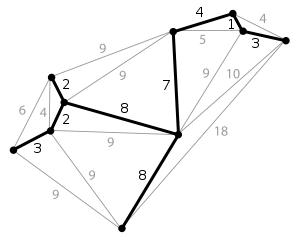
\includegraphics[width=.5\textwidth]{MST.png}
\end{frame}
\subsection{Use cases}

\begin{frame}
\frametitle{Input sets: G(100, 0.02)}
\begin{figure}
 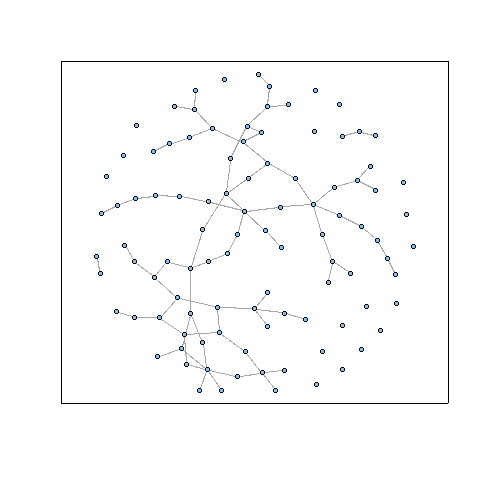
\includegraphics[width=.7\textwidth]{graphGNP.png}
\end{figure}
\end{frame}

\begin{frame}
\frametitle{Input sets: PA(100)}
\begin{figure}
 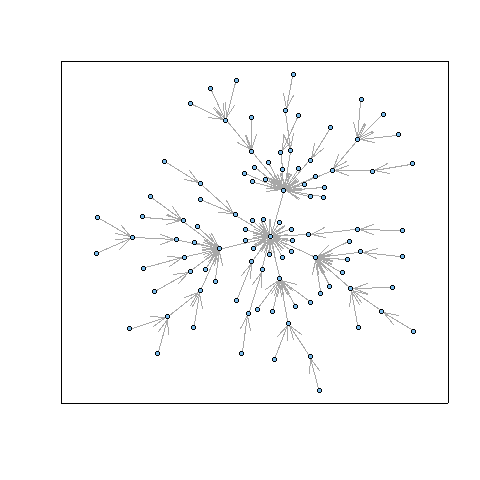
\includegraphics[width=.7\textwidth]{graphPA.png}
\end{figure}
\end{frame}

%%%%%%%%%%%%%%%%%%%%%%%%%%%%%%%%%%%%%%%%%%%%%%%%%%%%%%%%%%%%%%%%%%%%
% SECTION 2
%%%%%%%%%%%%%%%%%%%%%%%%%%%%%%%%%%%%%%%%%%%%%%%%%%%%%%%%%%%%%%%%%%%%

\section{Algorithms}
\subsection{Prim}
\begin{frame}
\frametitle{Sequential Prim}

    \begin{itemize}
        \item Initialise a tree with a single random vertex.
        \item Among all the edges connecting the tree to another vertex, find the minimum-weighted one and transfer it to the tree.
        \item Repeat until all vertices are in the tree.
    \end{itemize}

\end{frame}

\begin{frame}
\frametitle{Sequential Prim}

%% Adjacency matrix of graph
%% \  a  b  c  d  e  f  g
%% a  x  7     5
%% b  7  x  8  9  7
%% c     8  x     5
%% d  5  9     x 15  6
%% e     7  5 15  x  8  9
%% f           6  8  x 11
%% g              9  11 x

\tikzstyle{vertex}=[circle,fill=black!25,minimum size=20pt,inner sep=0pt]
\tikzstyle{selected vertex} = [vertex, fill=red!24]
\tikzstyle{edge} = [draw,thick,-]
\tikzstyle{weight} = [font=\small]
\tikzstyle{selected edge} = [draw,line width=5pt,-,red!50]
\tikzstyle{ignored edge} = [draw,line width=5pt,-,black!20]

\begin{figure}
\begin{tikzpicture}[scale=1.8, auto,swap]
    % Draw a 7,11 network
    % First we draw the vertices
    \foreach \pos/\name in {{(0,2)/a}, {(2,1)/b}, {(4,1)/c},
                            {(0,0)/d}, {(3,0)/e}, {(2,-1)/f}, {(4,-1)/g}}
        \node[vertex] (\name) at \pos {$\name$};
    % Connect vertices with edges and draw weights
    \foreach \source/ \dest /\weight in {b/a/7, c/b/8,d/a/5,d/b/9,
                                         e/b/7, e/c/5,e/d/15,
                                         f/d/6,f/e/8,
                                         g/e/9,g/f/11}
        \path[edge] (\source) -- node[weight] {$\weight$} (\dest);
    % Start animating the vertex and edge selection. 
    \foreach \vertex / \fr in {d/1,a/2,f/3,b/4,e/5,c/6,g/7}
        \path<\fr-> node[selected vertex] at (\vertex) {$\vertex$};
    % For convenience we use a background layer to highlight edges
    % This way we don't have to worry about the highlighting covering
    % weight labels. 
    \begin{pgfonlayer}{background}
        \pause
        \foreach \source / \dest in {d/a,d/f,a/b,b/e,e/c,e/g}
            \path<+->[selected edge] (\source.center) -- (\dest.center);
        \foreach \source / \dest / \fr in {d/b/4,d/e/5,e/f/5,b/c/6,f/g/7}
            \path<\fr->[ignored edge] (\source.center) -- (\dest.center);
    \end{pgfonlayer}
\end{tikzpicture}
\end{figure}

\end{frame}


\begin{frame}
    \frametitle{Sequential and parallel Prim}
    Sequential complexity:
    \begin{itemize}
        \item $O(V^{2})$: Adjacency matrix representation
        \item $O(E \log V)$: Adjacency list representation with the use of a binary heap
    \end{itemize}

    \visible<2>{We can parallelize the search of the edge of minimum weight by dividing the vertices and edges between processors to compute local minima.}

\end{frame}

\subsection{Kruskal}

\begin{frame}
    \frametitle{Sequential Kruskal}
    \begin{itemize}
        \item Sort all edges by growing weight.
        \item For each edge: Add it to the MST if it doesn't create a cycle.
    \end{itemize}

    \visible<2>{
        \begin{figure}
            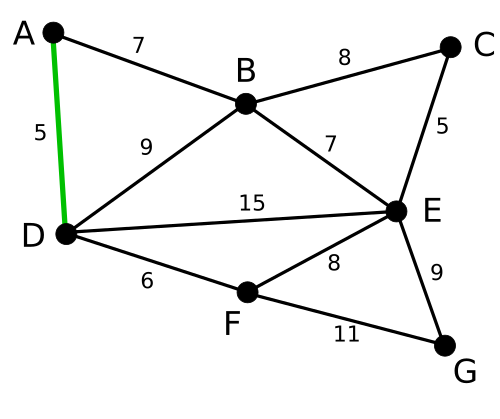
\includegraphics[width=.5\textwidth]{kruskal_1.png}
        \end{figure}
    }

\end{frame}

\begin{frame}
    \frametitle{Sequential Kruskal}
    \begin{itemize}
        \item Sort all edges by growing weight.
        \item For each edge: Add it to the MST if it doesn't create a cycle.
    \end{itemize}

    \begin{figure}
        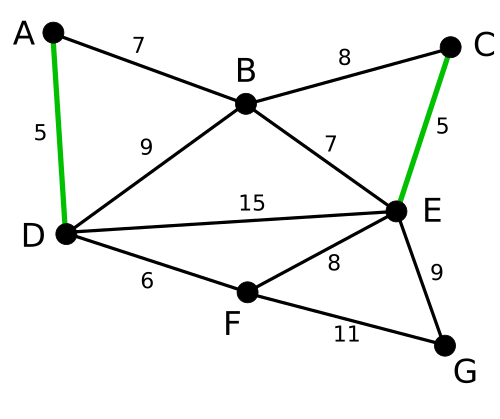
\includegraphics[width=.5\textwidth]{kruskal_2.png}
    \end{figure}

\end{frame}

\begin{frame}
    \frametitle{Sequential Kruskal}
    \begin{itemize}
        \item Sort all edges by growing weight.
        \item For each edge: Add it to the MST if it doesn't create a cycle.
    \end{itemize}

    \begin{figure}
        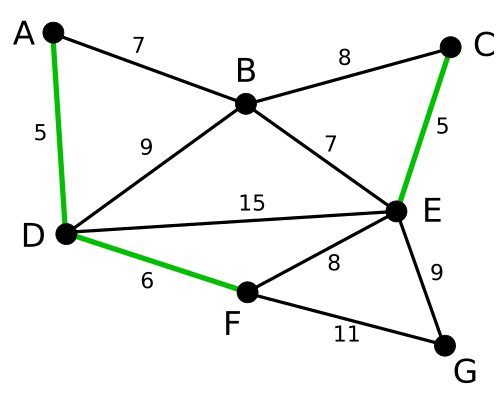
\includegraphics[width=.5\textwidth]{kruskal_3.png}
    \end{figure}

\end{frame}


\begin{frame}
    \frametitle{Sequential Kruskal}
    \begin{itemize}
        \item Sort all edges by growing weight.
        \item For each edge: Add it to the MST if it doesn't create a cycle.
    \end{itemize}

    \begin{figure}
        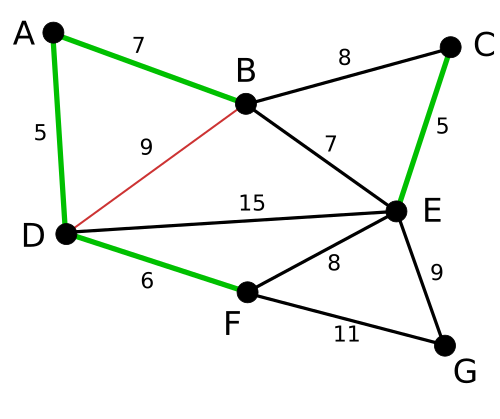
\includegraphics[width=.5\textwidth]{kruskal_4.png}
    \end{figure}

\end{frame}


\begin{frame}
    \frametitle{Sequential Kruskal}
    \begin{itemize}
        \item Sort all edges by growing weight.
        \item For each edge: Add it to the MST if it doesn't create a cycle.
    \end{itemize}

    \begin{figure}
        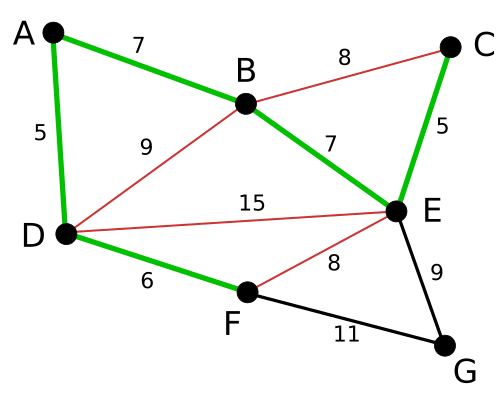
\includegraphics[width=.5\textwidth]{kruskal_5.png}
    \end{figure}

\end{frame}


\begin{frame}
    \frametitle{Sequential Kruskal}
    \begin{itemize}
        \item Sort all edges by growing weight.
        \item For each edge: Add it to the MST if it doesn't create a cycle.
    \end{itemize}

    \begin{figure}
        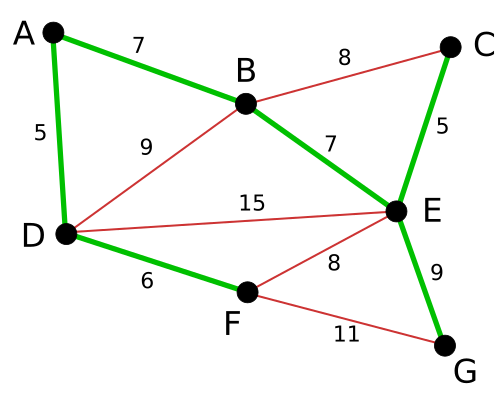
\includegraphics[width=.5\textwidth]{kruskal_6.png}
    \end{figure}

\end{frame}

\begin{frame}
    \frametitle{Data structure: Union-find}
    Represents the connected components of the graph given our MST.
    Implementation with an array $parent$ and 3 operations:
    \begin{itemize}
        \item Create: Every vertex is in its own component
            \begin{enumerate}
                \item $parent[x] = x$.
            \end{enumerate}
        \item<2-> Find(x): Find the component of this vertex.
            \begin{enumerate}
                \item If $parent[x] \neq x$, then $parent[x] = find(parent[x])$
                \item Return $parent[x]$.
            \end{enumerate}
        \item<3-> Union(x, y): Unite two components.
            \begin{enumerate}
                \item $parent[find(x)] = find(y)$.
            \end{enumerate}
    \end{itemize}

\end{frame}

\begin{frame}
    \frametitle{Sequential and parallel Kruskal}
    Sequential complexity:
    \begin{itemize}
        \item $O(E \log E)$: Sort all edges by growing weight.
        \item $O(E)$ (in practice): For each edge: Add it to the MST if it doesn't create a cycle.
    \end{itemize}

    \visible<2>{We can parallelize the sort on $O(\log E)$ processors: $O(E)$ (in practice).}

\end{frame}

\begin{frame}
    \frametitle{A better parallel approach: Filter-Kruskal}
    Similar to a quick sort\footcite{Osipov:2009:FMS:2791220.2791225}:
    \begin{enumerate}
        \item If $E < threshold$, solve using classical Kruskal
        \item Choose a pivot (edge)
        \item Partition in two sets $E_{\leq}, E_>$ (weight)
        \item Recursive call to solve problem with $E_{\leq}$
        \item Filter out the edges of $E_>$ that connect two vertices of the same component
        \item Recursive call to solve problem with $E_>$
    \end{enumerate}

    \visible<2>{Better for parallelization since we can distribute the edges for filtering and partitioning.}

\end{frame}

\subsection{Borůvka (Sollin)}
\begin{frame}[fragile]
\frametitle{Borůvka (Sollin)}
\begin{columns}
\begin{column}{.4\linewidth}
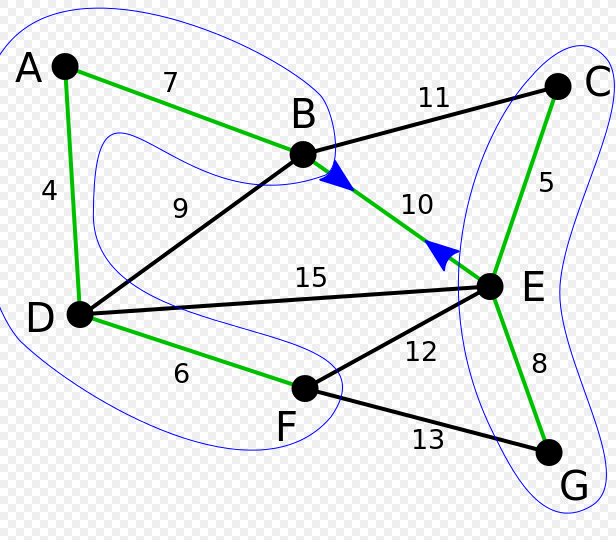
\includegraphics[scale=.22]{Sollin.png}
\end{column}

\begin{column}{.5\linewidth}
\begin{verbatim}
1) Init V as independant sets.
2) Initialize MST as empty.
3) While #sets > 1, do:
  a)  Find closest E 
      from this set to another.
  b)  Add this E to MST 
      if not already added.  
4) Return MST.
\end{verbatim}
\end{column}
\end{columns}
\footcite{chung1996parallel}
\footcite{bader2006fast}
\end{frame}

\subsection{Others}
\begin{frame}
\begin{columns}
\begin{column}{.5\linewidth}
\begin{itemize}
\item[•] Prim (Parallel \& Seq)
\item[•] Kruskal (Parallel \& Seq),\\Kruskal filter
\item[•] Sollin (Parallel \& Seq)
\end{itemize}
\hfill
\hrulefill
\hfill
\begin{itemize}
\item[•] Randomization
\end{itemize}
\hfill
\hrulefill
\hfill
\begin{itemize}
\item[•] Correctness
\end{itemize}
\hfill
\end{column}
\begin{column}{.5\linewidth}
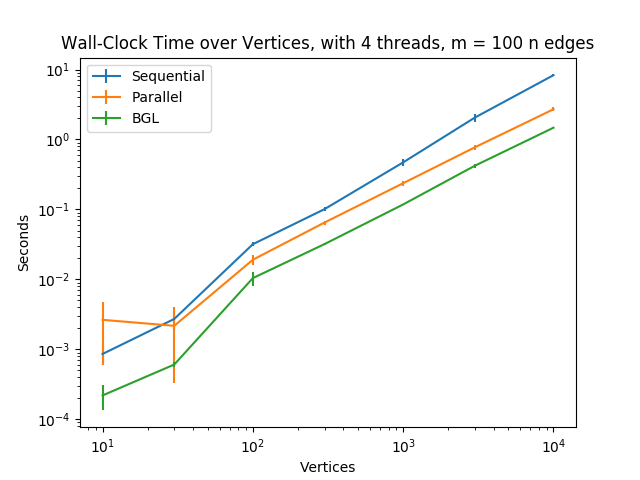
\includegraphics[scale=.23]{Bench.png}
\end{column}
\end{columns}
\end{frame}
%%%%%%%%%%%%%%%%%%%%%%%%%%%%%%%%%%%%%%%%%%%%%%%%%%%%%%%%%%%%%%%%%%%%
% SECTION 3
%%%%%%%%%%%%%%%%%%%%%%%%%%%%%%%%%%%%%%%%%%%%%%%%%%%%%%%%%%%%%%%%%%%%

\section{Environment}
\begin{frame}
\frametitle{Architecture}
\begin{figure}
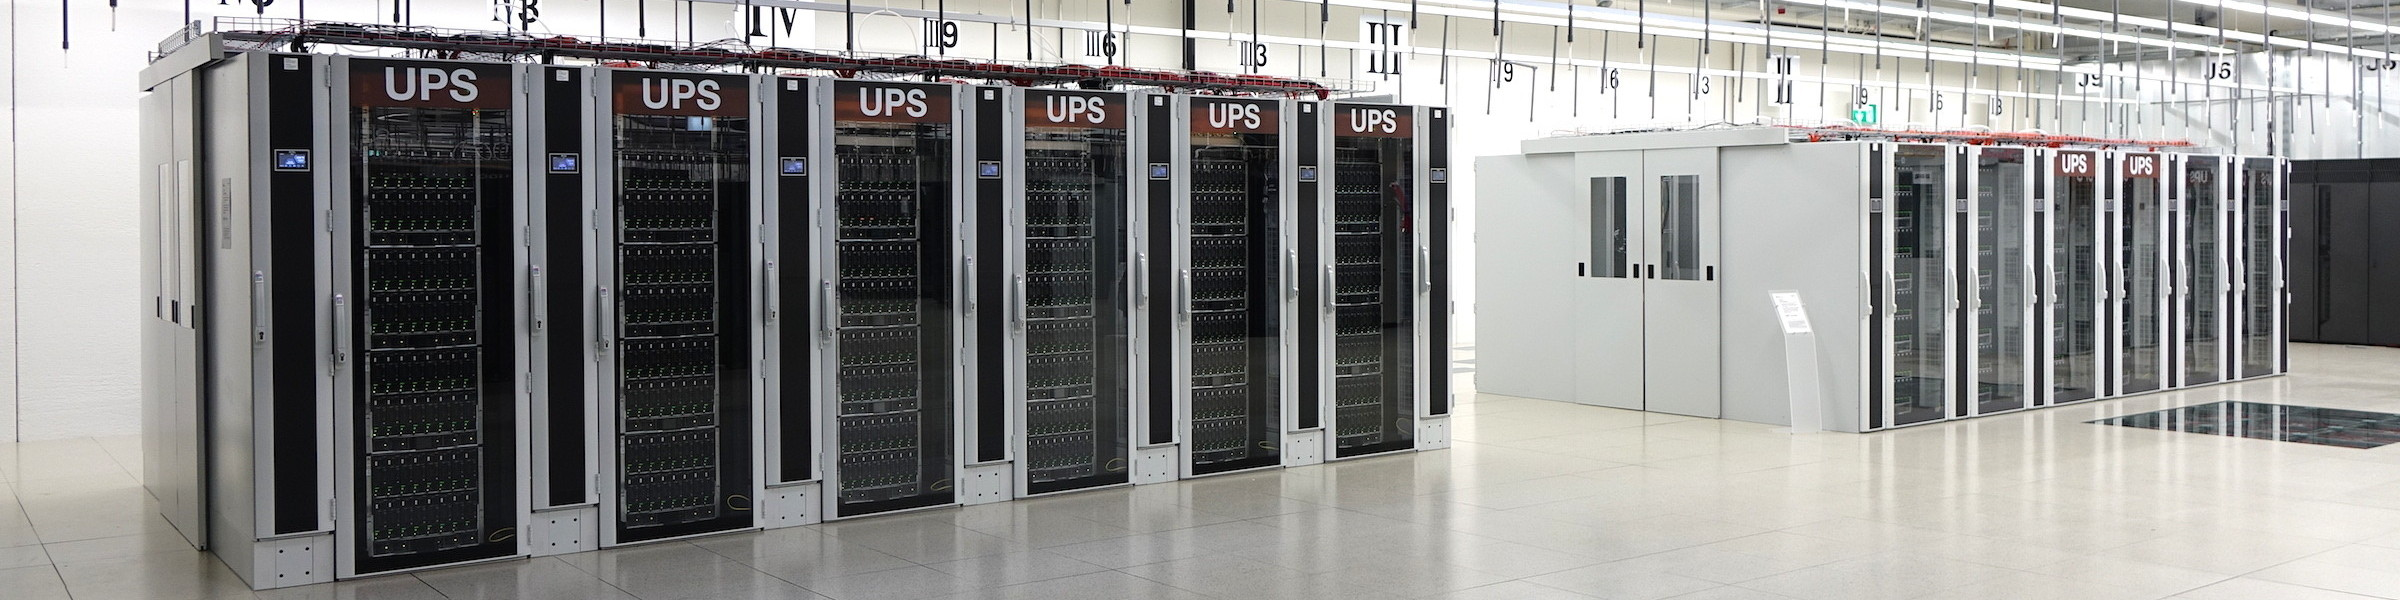
\includegraphics[scale=0.4]{EULER.jpg}
\end{figure}

\centering{ \large EULER Cluster }

\vspace{.5 cm}

Xeon E$x, x\in\{3, 5, 7\}$\\x86\_64 architecture
\vfill
{
\tiny
Source : 
\url{https://scicomp.ethz.ch/wiki/Euler}
}
\end{frame}
\begin{frame}
\frametitle{Tools}
\begin{columns}
\begin{column}{.4\linewidth}

\includegraphics[scale=.1]{OPENMP.png}
\end{column}

\begin{column}{.6\linewidth}
\begin{itemize}
\item[•] CMake\\\hspace{.5cm}v3.3+
\vspace{.2cm}
\item[•] C++11\\\hspace{.5cm}GCC v4.9.2+
\vspace{.2cm}
\item[•] OpenMPI (shared memory)\\\hspace{.5cm}v1.6.5+
\end{itemize}
\end{column}
\end{columns}

\end{frame}

%%%%%%%%%%%%%%%%%%%%%%%%%%%%%%%%%%%%%%%%%%%%%%%%%%%%%%%%%%%%%%%%%%%%
% SECTION 4
%%%%%%%%%%%%%%%%%%%%%%%%%%%%%%%%%%%%%%%%%%%%%%%%%%%%%%%%%%%%%%%%%%%%

\section{Benchmarking}
\subsection{Reference, baseline, tools}
\begin{frame}

\textbf{\Large Tools} 

\begin{itemize}
\item[•] \textbf{Measures :} LibSciBench library
\item[•] \textbf{Interpretation :} 
\begin{itemize}
\item[•] LibSciBench's R scripts
\item[•] (Custom python scripts)
\end{itemize}
\end{itemize}

{
\tiny
Ref : 
\url{https://spcl.inf.ethz.ch/Research/Performance/LibLSB/}
}

\vfill

\textbf{\Large Baseline}

\begin{columns}
\begin{column}{0.3\linewidth}
\begin{center}
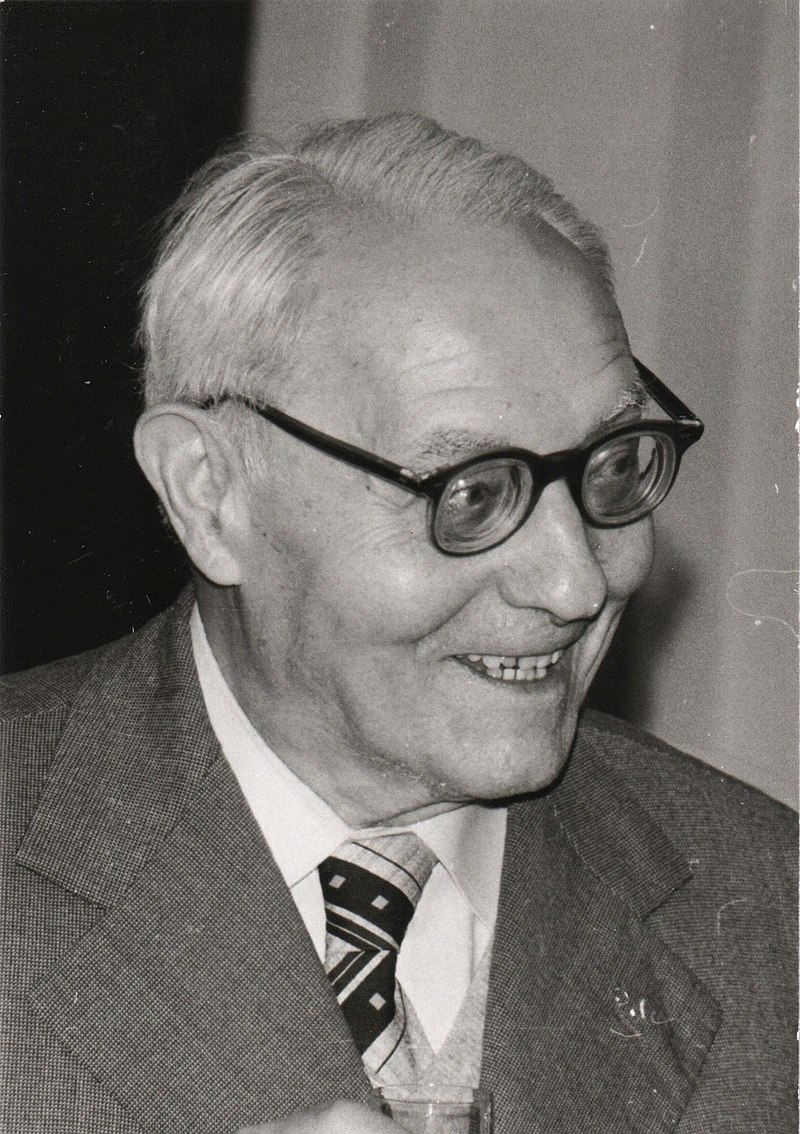
\includegraphics[scale=.05]{Boruvka.jpg}
\end{center}
\end{column}
\begin{column}{0.7\linewidth}
\begin{center}
Borůvka's serial algorithm

$O(E \cdot log(V))$
\end{center}
\end{column}
\end{columns}
{\tiny \url{https://en.wikipedia.org/wiki/Otakar_Bor\%C5\%AFvka}}



\end{frame}

\begin{frame}
    \printbibliography
\end{frame} 



\end{document}
